\section{Consequences Downstream}
\label{sec:downstream}

\begin{table*}[t]
    \centering
    \small
    \begin{tabular}{@{}lrr ccc ccc@{}}
\toprule
 & \multicolumn{2}{c}{Detections} & \multicolumn{3}{c}{Accepted by SAM 3 (\%)} & \multicolumn{3}{c}{AUROC, correct vs.\ class-absent} \\
\cmidrule(lr){2-3}\cmidrule(lr){4-6}\cmidrule(l){7-9}
Detector, images & all & class-absent & absent & absent, gated & correct, gated & detector & SAM 3 & SAM 3, gated \\
\midrule
Faster R-CNN, COCO set & 3,122 & 536 & 100.0 & 60.8 & 99.9 & 0.919 & 0.665 & 0.960 {\scriptsize[0.948, 0.972]} \\
Faster R-CNN, held-out & 3,152 & 565 & 99.8 & 57.9 & 99.9 & 0.932 & 0.646 & 0.961 {\scriptsize[0.949, 0.971]} \\
RetinaNet, COCO set & 2,767 & 326 & 99.7 & 59.8 & 99.9 & 0.896 & 0.571 & 0.958 {\scriptsize[0.944, 0.972]} \\
\bottomrule
\end{tabular}

    \caption{\textbf{\sam{} as a verifier of detector boxes.}
    Each detection is passed as a positive exemplar with its class name as the phrase, and is accepted when a mask is kept.
    \emph{Class-absent} (\emph{absent} in the column heads): the class has no COCO ground truth in the image.
    \emph{Gated} acceptance uses the hard gate at $\tau = 0.10$.
    AUROC ranks correct against class-absent detections by the detector's confidence, by \sam{}'s best score, and by \sam{}'s best score with the text-only presence substituted (gated).
    The two COCO-set rows use the same images; the held-out row shares none with them.}
    \label{tab:detector}
\end{table*}

\begin{figure}[t]
    \centering
    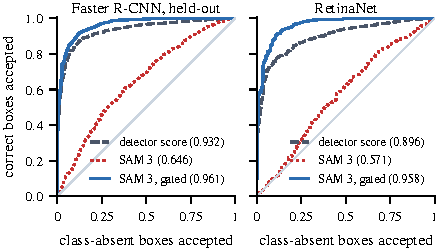
\includegraphics[width=\linewidth]{fig/roc.pdf}
    \caption{\textbf{Correct against class-absent detections.}
    ROC curves for the three scores of \cref{tab:detector}; AUROC in the legend.
    Without the gate \sam{} assigns nearly every box a high score.}
    \label{fig:roc}
\end{figure}

\subsection{Verifying detector boxes}
\label{sec:detector}

A common pipeline lets a detector propose boxes and a segmenter turn them into masks~\cite{ren2024groundedsam}.
With \sam{} one would pass each box as a positive exemplar with the detector's class as the phrase, and expect the concept model to drop boxes whose class is not there.
We ran Faster R-CNN~\cite{ren2015faster} and RetinaNet~\cite{lin2017focal}, both with torchvision's COCO-trained ResNet-50 FPN v2 weights, kept detections with a score of at least 0.30, at most eight per image, and labelled a detection \emph{correct} when it has an IoU of at least 0.5 with a ground-truth box of its class and \emph{class-absent} when the image has no ground truth of that class.
Both detectors were run on the COCO set of \cref{sec:setup}, and Faster R-CNN again on the next 500 val2017 images that share none with it.
One image in each Faster R-CNN run produced no detection above the score threshold, so the table covers 499 images per run.
Of the 499 held-out images, 46 belong to the LVIS selection set on which $\tau$ was chosen.

\paragraph{Without the gate \sam{} verifies nothing.}
It accepts 100\%, 99.8\% and 99.7\% of class-absent detections in the three runs of \cref{tab:detector}, and all correct ones.
Its best score ranks correct above class-absent boxes with an AUROC of 0.57--0.66, far below the detectors' own confidence at 0.90--0.93.

\paragraph{With the text-only presence it is the better scorer.}
Substituting $\ptext$ in \cref{eq:score} lifts the AUROC to 0.960, 0.961 and 0.958.
The paired gain over the detector's confidence is 0.042 [0.029, 0.055] for Faster R-CNN on the COCO set, 0.029 [0.016, 0.042] on held-out images, and 0.063 [0.043, 0.082] for RetinaNet (\cref{fig:roc}).
The criterion on this AUROC was preregistered for the RetinaNet and held-out runs after the first Faster R-CNN run produced 0.960.

\paragraph{What the gate does not fix.}
As a decision, the hard gate at $\tau = 0.10$ keeps 99.9\% of correct detections and still accepts 58--61\% of class-absent ones.
Our phase-2 criterion asked the multiplicative gate for a 70\% relative drop; it gave 61.0\% and failed.
The reason is in the text-only head: it believes the class is present for 36--40\% of class-absent detections, against 1.6\% for LVIS-verified absent phrases.
A detector's mistake is not a random phrase.
It is a class the scene suggests (bottle, person, dining table and car are among the six most frequent residual classes in all three runs), and ``absent'' here only means that COCO has no label.
After the fact, we checked the first run's class-absent boxes against LVIS annotations of the same images, under the multiplicative gate: 6.9\% of the 204 boxes the gate accepted match an LVIS instance of a corresponding category at a box IoU of 0.5, against 0.9\% of the 321 it rejected.
Unlabelled real objects explain a small part of the residual.
The rest we cannot resolve without human labels, which we did not collect.
The gate is also blind to localization.
When the wrong detections of classes that \emph{are} in the image are included, the gated score reaches an AUROC of 0.81--0.83 against 0.87--0.90 for the detector's confidence, because presence is an image-level statement and says nothing about a misplaced box.

\subsection{Counting with an exemplar}
\label{sec:counting}

\begin{table}[t]
    \centering
    \small
    \begin{tabular}{@{}lcc@{}}
\toprule
Prompt & MAE, true class & False count (\%) \\
\midrule
text only & 34.08 & -- \\
text + box & 28.73 & 85.5 {\scriptsize[82.0, 89.0]} \\
text + box, hard gate & 29.27 & 4.3 {\scriptsize[2.3, 6.5]} \\
\bottomrule
\end{tabular}

    \caption{\textbf{FSC-147, 400 test images.}
    The count is the number of kept masks; the box is the image's first exemplar box.
    \emph{False count}: at least one mask is kept when the phrase is another FSC-147 class name, drawn with a fixed seed, that does not describe the image.}
    \label{tab:count}
\end{table}

Exemplar-based counters are prompted with a box around one instance~\cite{ranjan2021fsc}.
We prompt \sam{} with an FSC-147 class name that does not describe the image and the image's first exemplar box.
It reports at least one object in 85.5\% of images [82.0, 89.0], with presence non-negative in 94.8\%; for the same class names alone, presence is non-negative in 0.5\% (\cref{tab:count}).
The hard gate reduces false counts to 4.3\% [2.3, 6.5].
On the true class, the gate changes the mean absolute error from 28.73 to 29.27, a cost of 0.55 [0.23, 0.93] that comes from the 3.5\% of images whose true class the text-only pass rejects.
\sam{} is not a strong counter on this benchmark under any prompt, and its errors are dominated by dense images (the median ground-truth count is 31 and the mean 63.8).
The \sam{} paper does not use the presence score when counting~\cite{carion2026sam3}; we keep \cref{eq:score} throughout so that the conditions are comparable.
The absent class names are not verified by annotation.
